\documentclass{article}
\usepackage{geometry}
 \geometry{
 a4paper,
 %total={170mm,257mm},
 %left=25.4mm,
 %top=25.4mm,
 %bottom=25.4mm,
 %right=25.4mm,
 }

\usepackage[utf8]{inputenc}
\usepackage{amsmath,amsthm,amssymb,graphicx,mathtools,tikz,hyperref}
\usepackage[round]{natbib}
\usepackage{listings}
\usepackage{graphicx}
\usepackage{booktabs}

\graphicspath{ {../figures/} }

\title{Analytical approximations for leave one out utility standard errors}
\author{Leevi Lindgren \footnote{I thank Aki Vehtari and Nikolas Siccha for their comments.}}
\date{\today}

\begin{document}

\maketitle

\clearpage
\section*{Note}
The approach in this report was motivated by the work by \cite{hastings1970monte} who proposes an approximation for the variance of the ratio of two random variables. However, the formula provided by \cite{hastings1970monte} contains two typos: on page 8, in the formula for the variance of the ratio, $\bar{Z}$ is missing the "bar" symbol and computed variance $s_{\bar{Z}}$ is missing the second power. The missing second power caused the author of this report to mistake it for the standard deviation instead of variance, which was followed by weird simulation results. Unfortunately, research papers are not like software: you cannot make a pull request to fix a bug.
\clearpage

\tableofcontents
\clearpage
\section{Introduction}

This report presents analytical approximations for standard errors of different predictive metrics in the context of Bayesian predictive model assessment. 

Usefulness of a statistical model is often evaluated by assessing the predictive performance of the model. Significant discrepancies between the predicted values and observations suggest that the model is not useful, even though the ultimate goal is to make inference in some parameter, such as treatment effect. There is a major challenge when evaluating the predictive power: future observations are not available.

Predictive performance of a statistical model is hence estimated as the expected predictive predictive performance (or utility). 

Introduce LOO

Discuss comparison using LOO utilities

Discuss the uncertainty evaluation of the estimation. Why this analytical approximation approach would be useful (compared to e.g. BB)?

The report is structured as follows: The second section follows closely the ideas presented in \cite{vehtari_survey_2012} and introduces briefly some theory on model assessment and comparison based on predictive performance. Third section presents Taylor approximation for functions of two variables, and shows how expectations and variances can be approximated when the variables are considered to be random. Four section discusses X different metrics and the analytical formulas for the variance of the estimator. Moreover, approximation of variance of the difference between two estimators is also represented. In section five, we verify the validity of the approximations with simulation studies. Finally, the last section provides concluding remarks.

\section{Predictive methods for Bayesian model assessment}
This section reviews three concepts central to the later discussion in the paper: 1) estimating the predictive performance of a statistical model 2) comparing statistical models and 3) quantifying the uncertainty in the performance estimates. We follow closely the ideas from \cite{vehtari_survey_2012}. Notation through out this report, and specifically this section, is summarized in Table  \ref{tab:notation}.

\subsection{Estimating the predictive performance}
As noted in the first section, the usefulness of a statistical model is often evaluated on the basis of predictive performance. Performance is measured by some utility function $u$. Formally, the expected predictive performance for utility $u$ can be written as 
\begin{equation}
u(M_k | y) = \int u(M_k, \hat{a}_k, \tilde{y} | y) p_t(\tilde{y}) d\tilde{y}, \label{eq:true-utility}
\end{equation}
where $\hat{a}_k$ denotes the optimal decision under $M_k$. For example, if the defined utility is mean squared error (MSE), the optimal decision, or prediction, is using the posterior predictive expectation of $\tilde{y}$, i.e., $E\left[ \tilde{y} | y, M_k \right]$. Then Equation \eqref{eq:true-utility} for MSE can be written as
$$
u^{\text{MSE}}(M_k | y) = \int \left( \tilde{y} - E\left[ \tilde{y} | y, M_k \right] \right)^2 p_t(\tilde{y}) d\tilde{y}
$$

Computing \eqref{eq:true-utility} poses a challenge as we rarely know the true mechanism which generates the data, $p_t(y)$. In optimal case we would have independent test data $\tilde{y}_i, i=1,...,\tilde{n}$ and \eqref{eq:true-utility} would be easy to compute using
\begin{equation}
    \hat{u}_{\text{test}}(M_k | y) = \frac{1}{\tilde{n}} \sum_{i=1}^{\tilde{n}} u(M_k, \hat{a}_k, \tilde{y}_i | y). \label{eq:test-utility}
\end{equation}
However, typically we don't have access to such data.

To tackle this, naive approach would be to re-use the observed data which was used to train the model, and compute "training" version of \eqref{eq:true-utility}:
\begin{equation}
    \hat{u}_{\text{train}}(M_k | y) = \frac{1}{n} \sum_{i=1}^n u(M_k, \hat{a}_k, y_i | y). \label{eq:train-utility}
\end{equation}
Training utility in \eqref{eq:train-utility} is a biased estimate of \eqref{eq:true-utility}, and typically is over optimistic about the predictive performance of the model.

One way to improve the quality of the training utility estimate is to introduce a sample re-use strategy in which data is split into folds $I_1, ..., I_K$ and each dataset $y_{I_k}$ is used in turn as a validation set, while model is trained with $y_{-I_k}$. This approach is called cross-validation (CV). Special case of CV is leave-one-out corr-validation (LOO-CV), where data of size $n$ is split into $n$ folds. LOO-CV utility estimate is then given as 
\begin{equation}
    \hat{u}_{\text{LOO}}(M_k | y) = \frac{1}{n} \sum_{i = 1}^n u(M_k, \hat{a}_k, y_i | y_{-i}) \label{eq:loo-utility}.
\end{equation}

\subsection{Model comparison}
Typically in Bayesian workflow, the modeller has multiple candidate models. If model averaging is not possible or the set of candidate models need to be thinned, e.g. due to the cost of data gathering, she would like to choose one model from the set of candidates. The goal is to choose model having the best expected utility.

Ideas from the previous section can be extended into the context of model comparison. Consider two models, $M_A$ and $M_B$. With a slight use of notation, we write the difference on the expected utility between models A and B as
\begin{align}
    u(M_A, M_B | y) &= u(M_A | y) - u(M_B | y) \nonumber \\ 
    &= \int u(M_A, \hat{a}_k, \tilde{y} | y) p_t(\tilde{y}) d\tilde{y} - \int u(M_B, \hat{a}_k, \tilde{y} | y) p_t(\tilde{y}) d\tilde{y} \nonumber \\
    &= \int \left( u(M_A, \hat{a}_k, \tilde{y} | y) - u(M_B, \hat{a}_k, \tilde{y} | y) \right) p_t(\tilde{y}) d\tilde{y}
\end{align}

Following the ideas from the previous section, we can compute the estimators for the difference in utilities given e.g. independent test data, training data or LOO re-use of data. As we will focus on LOO estimators in the following sections, we only state LOO estimator for the difference:
\begin{align}
    \hat{u}_{\text{LOO}}(M_A, M_B | y) &= \frac{1}{n} \sum_{i=1}^n u(M_A, \hat{a}_k, y_i | y_{-i}) - \frac{1}{n} \sum_{i=1}^n u(M_A, \hat{a}_k, y_i | y_{-i}) \nonumber \\
    &:= \frac{1}{n}\sum_{i=1}^n u(M_A, M_B, y_i | y_{-i})
\end{align}



\subsection{Assessing the uncertainty of the estimators}
If we knew $p_t(y)$, we could compute the quantity \eqref{eq:true-utility} with arbitrary accuracy and there would be no uncertainty. If we had an independent testdata, then the uncertainty could be quantified with the Monte Carlo standard error of \eqref{eq:test-utility}. 

However, for particular utilities, such root mean squared error (RMSE) and (Bayesian) R-squared, we "loose" the information of individual terms. Take the RMSE as an example. It is defined as the square root of the mean squared error, so we don't have the individual utility terms $u(M_k, \hat{a}_k, y_i | \cdot)$

Alternatively, we could use some other approach, such as Bayesian bootstrap (\cite{rubin_bayesian_1981}, \cite{vehtari_bayesian_2002}, \cite{vehtari_survey_2012}).

\begin{table}[]
    \centering
    \begin{tabular}{l | p{0.8\linewidth}}
    \toprule
        notation & meaning \\ \midrule
        $p_t(\tilde{y})$ & The "true" data generating distribution, which is typically unknown. \\
        $y_i | y_{-i}$ & $y_i$ given all other observations than $y_i$. E.g. $p(y_i | y_{-i})$ denotes the leave one out predictive distribution of $y_i$. \\
        $ u(M_k | y) $ & Utility for model $M_k$ with respect to the true data generating process given the observed data $y_i$. \\
        $u(M_k, y_i | y)$ & Utility for a single data point, if applicable
        
    \end{tabular}
    \caption{Notation used throughout the paper.}
    \label{tab:notation}
\end{table}

\section{Taylor approximation for a function of two variables}

Let $f(x, y): \mathbb{R}^2 \rightarrow \mathbb{R}$ be a function of two (random) variables. The first order Taylor approximation of a function of two variables around point $x_0, y_0$ is given by
\begin{align}
    f(x, y) &\approx f(x_0, y_0) + \frac{\partial }{\partial x} f(x_0, y_0) (x - x_0) + \frac{\partial }{\partial y} f(x_0, y_0) (y - y_0) \label{tapprox}
\end{align}

Now, let's take two random variables $X$ and $Y$ and do the approximation around the expected values $(\mu_X, \mu_Y)$ = $(E[X], E[Y])$. Using \eqref{tapprox} we get
\begin{align}
    f(X, Y) \approx f(\mu_X, \mu_Y) + \frac{\partial }{\partial x} f(\mu_X, \mu_Y) (X - \mu_X) + \frac{\partial }{\partial y} f(\mu_X, \mu_Y) (Y - \mu_Y) \label{rvtapprox}
\end{align}

\subsection{Taylor approximation for the expected value}
Given that terms containing partial derivatives in \eqref{rvtapprox} go to zero under expectation, we get the following, simple, first order approximation for the expected value of $f(X, Y)$:
\begin{align}
    E[f(X, Y)] \approx f(\mu_X, \mu_Y) \label{eapprox}
\end{align}

\subsection{Taylor approximation for variance}
For variance
\begin{align}
    \text{var}(f(X, Y)) &= E\left[ \left(f(X, Y) - E[f(X,Y)] \right)^2 \right] \nonumber \\
    &\approx E\left[ \left( f(X, Y) - f(\mu_X, \mu_Y) \right)^2 \right] \nonumber
\end{align}
Next, we plug in \eqref{rvtapprox} for $f(X,Y)$ which yields (we write $\frac{\partial }{\partial x} f(\mu_X, \mu_Y) = \frac{\partial f}{\partial x}$ for notational simplicity):
\begin{align}
    \text{var}(f(X, Y)) &\approx E\left[ \left( \frac{\partial f}{\partial x} (X - \mu_X) + \frac{\partial f}{\partial y} (Y - \mu_Y) \right)^2 \right] \nonumber \\
    &= E\left[ \left( \frac{\partial f}{\partial x}  \right)^2 (X - \mu_X)^2 + 2 \frac{\partial f}{\partial x} \frac{\partial f}{\partial y} (X - \mu_X)(Y - \mu_Y) + \left( \frac{\partial f}{\partial y}  \right)^2 (Y - \mu_Y)^2  \right] \nonumber \\
    &= \left( \frac{\partial f}{\partial x}  \right)^2 \text{var}(X) + 2 \frac{\partial f}{\partial x} \frac{\partial f}{\partial y} \text{cov}(X, Y) + \left( \frac{\partial f}{\partial y}  \right)^2 \text{var}(Y) \label{varapprox}
\end{align}

\section{Approximations for standard errors of LOO utilities}
In what follows, we consider general setting, where we have $n$ observations $(y_i, x_i)$ in which $x_i \in \mathbb{R}^p$ and $y_i \in \mathbb{R}$. We are estimating some utility $u(M_k | y)$ with $\hat{u}(M_k |y)$ computed from the sample.


\begin{table}[]
    \centering
    \begin{tabular}{l c c p{0.4\linewidth}}
    \toprule
    $u(M | y)$ & $\widehat{Var}(u)$  & $\widehat{Var}(u(M_A, M_B))$ & Comment \\ \midrule
    MAE & & \\
    MSE & & \\
    RMSE  & & \\
    $R^2$ & Equation \eqref{eq:loor2-se} & & $R^2$ is expressed in terms of ratio of two mean squared errors and Taylor approximation is used.
    \end{tabular}
    \caption{Taylor approximations for the standard error estimators of different utilities. The middle column refers to the equation of standard error estimator. The equations for standard error estimator for the difference between two utilities are reported in the right-most column.}
    \label{tbl:se-approximations}
\end{table}

\subsection{Mean absolute error}
The first metric we consider is mean absolute error (MAE).
\begin{equation}
    u(M_k | y)_{\text{MAE}} = \int \left| \tilde{y} - E\left[ \tilde{y} \right| y, M_k \right] | p_t(\tilde{y}) d\tilde{y}.
\end{equation}
We can estimate this quantity by in-sample estimator
\begin{equation}
    \hat{u}(M_k | y)_{\text{MAE}} = \frac{1}{n} \sum_{i=1}^n \left| y_i - E\left[ y_i | y, M_k \right] \right|,
\end{equation}
or by leave-one-out estimator
\begin{equation}
    \hat{u}(M_k | y)_{\text{LOO-MAE}} = \frac{1}{n} \sum_{i=0}^n \left| y_i - E\left[ y_i | y_{-i}, M_k \right] \right|
\end{equation}

\subsection{Root mean squared error}

\subsection{R-squared}
R-squared, or R2, is a typical measure used to assess how well a model fits data. \cite{gelman_r-squared_2019} propose a Bayesian version of the R2 as the classical R2 might get values larger than 1 for Bayesian regression models. See details from the paper. A nice property of Bayesian R2 is that we get a distribution of R2 values "for free", as it is computed using posterior predictive mean values of the model. This means that we can quantify the uncertainty of the estimator easily.

If (Bayesian) R2 is computed from the same data that was used to fit the model, it will give an overestimate of the predictive performance on a new, unobserved data. As often we don't have independent test data, we can use cross-validation to estimate the out-of-sample behavior of the R2. \cite{vehtari_practical_2016} propose an efficient and stable method for leave-one-out cross-validation using Pareto smoothed importance sampling. In the paper, log predictive density is used as the utility describing the predictive performance, but the method can easily be extended for other utilities as well, such as R2.

After computing LOO-R2 estimate, we want to quantify the uncertainty of the estimator. The uncertainty in LOO-R2 comes from not knowing the future data distribution \citep{vehtari_survey_2012}. One way to do it is to use Bayesian bootstrap \citep{rubin_bayesian_1981}. However, this report describes how to quantify the uncertainty using an analytical Taylor approximation approach.

The idea is to note that LOO-R2 is defined as a function of a ratio of two random variables. We can then use Taylor approximation of the function and the mean, variance, and covariance of the two random variables to approximate the standard error of the LOO-R2 estimator. 

LOO-R2 is defined as
\begin{align}
\text{R2}_{loo} = 1 - \frac{\text{var}(\hat{e}_{loo}) }{ \text{var}(y)} \label{loor2}
\end{align}

where $\hat{e}_{loo} = y - \hat{y}_{loo}$. Note that the nominator and denominator of the second term in \eqref{loor2} can be interpreted as the mean squared error of the LOO predictions and mean squared error of predicting the data with its mean, respectively. So we write \eqref{loor2} as 
\begin{align}
    \text{R2}_{loo} = 1 - \frac{\text{MSE}_{\hat{e}} }{ \text{MSE}_y} \label{mser2}
\end{align}

We can then compute the estimator for the variance of both using the same approach as in \cite{sivula_uncertainty_2022} and \cite{vehtari_practical_2016}:
\begin{align}
    \text{var}(\text{MSE}_{\hat{e}}) &= \frac{1}{n (n-1)} \sum_{i = 1}^n \left( \hat{e}_{loo, i}^2 - \text{MSE}_{\hat{e}} \right)^2 \label{vare}
\end{align}
and
\begin{align}
    \text{var}(\text{MSE}_y) &= \frac{1}{n (n-1)} \sum_{i = 1}^n \left( (y_i - \hat{y})^2 -\text{MSE}_y \right)^2 \label{vary},
\end{align}
where $\bar{y}$ is the sample mean of observations $y$. 

To utilize the Taylor approximation, we need to compute partial derivatives of function $f(x,y) = 1 - \frac{x}{y}$. With a simple calculus, we get
\begin{align}
    \frac{\partial}{\partial x}f(x,y) = -\frac{1}{y} \\
    \frac{\partial}{\partial y}f(x,y) = \frac{x}{y^2}.
\end{align}

Substituting these into \eqref{varapprox} yields
\begin{align}
    \text{var}(f(X, Y) \approx \frac{1}{\mu_Y^2} \left( \text{var}(X) - 2 \frac{\mu_X}{\mu_Y} \text{cov}(X,Y) + \left( \frac{\mu_X}{\mu_Y} \right)^2 \text{var}(Y) \right) \label{ratiovar}.
\end{align}

 To use this expression for the mean squared errors, we also need the covariance between $\text{MSE}_{\hat{e}}$ and $\text{MSE}_y$. This can be estimated in a similar way as the variances:
 \begin{align}
     \text{cov}(\text{MSE}_{\hat{e}}, \text{MSE}_{y} ) = \frac{1}{n (n -1 )} \sum_{i = 1}^n \left( \hat{e}_{loo, i}^2 - \text{MSE}_{\hat{e}} \right) \left( (y_i - \hat{y})^2 -\text{MSE}_y \right) \label{cov}.
 \end{align}
 
 Putting all pieces together, variance, and consequently the standard error, of LOO-R2 estimator can then be approximated by letting $\mu_X = \text{MSE}_{\hat{e}}$ and $\mu_Y = \text{MSE}_y$ and then substituting with \eqref{vare}, \eqref{vary} and \eqref{cov} into \eqref{ratiovar}:
 \begin{align}
     \text{var}(\text{R2}_{loo}) &= \frac{1}{\text{MSE}_y^2} \left( \text{var}(\text{MSE}_{\hat{e}}) - 2 \frac{\text{MSE}_{\hat{e}}}{\text{MSE}_y} \text{cov}(\text{MSE}_{\hat{e}}, \text{MSE}_{y} ) +  \left( \frac{\text{MSE}_{\hat{e}}}{\text{MSE}_y} \right)^2 \text{var}(\text{MSE}_y) \right) \label{eq:loor2-se}.
 \end{align}
 
\section{Simulation experiments}
We use simple simulation experiments to illustrate the behaviour of the proposed estimators for the variance. These simulation are by no means exhaustive, and more elaborate experiments are needed to verify the validity of the Taylor approximation method. We study the properties of the Taylor approximation of the variance of the estimator, and Taylor approximation of the variance of the difference when the utility is either RMSE or R-squared.

The procedure is as follows:

\subsection{RMSE}
\begin{figure}[!htb]
    \centering
    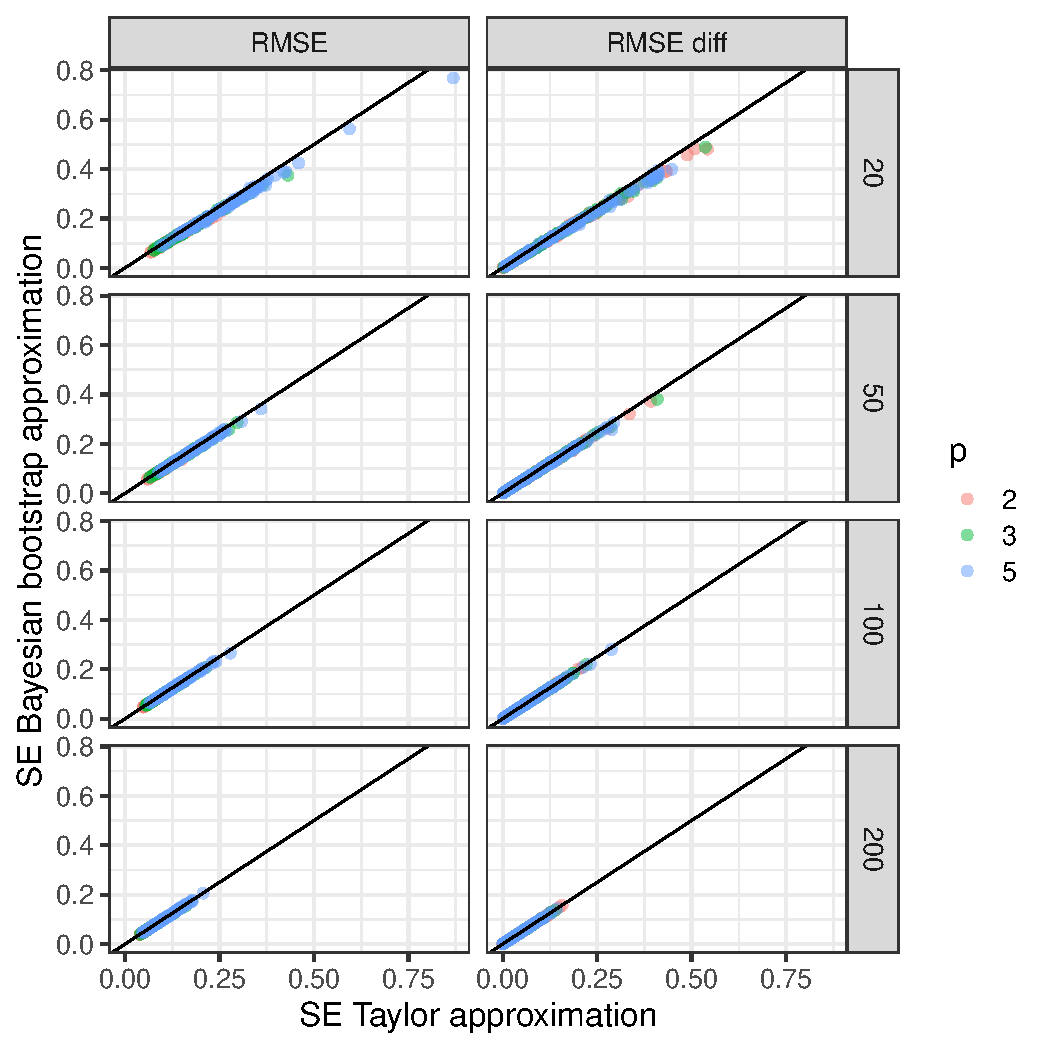
\includegraphics[width=\textwidth]{figures/rmse.pdf}
    \caption{Comparison of Taylor (x-axis) and Bayesian bootstrap (y-axis) approximations. Left panel shows the variance estimator for the RMSE estimator \eqref{eq:rmse} and right panel the variance estimator of the RMSE difference \eqref{eq:rmse-diff}.}
    \label{fig:rmse-plot}
\end{figure}


\subsection{LOO-R2}
To illustrate behaviour of the approximation for LOO-R2 standard error, we run a set of simulations with a few different configurations. We proceed as follows: choose number of observations $n$, number of predictors $p$ and observational noise $\sigma$ and then, draw predictor matrix $X \in \mathbb{R}^{n \times p}$ and $\beta \in \mathbb{R}^{p}$ from $N(0, 1)$ and  $\epsilon \in \mathbb{R}^{n}$ from $N(0, \sigma^2)$. Then we compute $y = X \beta + \epsilon$ for which we with linear model using R-package rstanarm \citep{rstanarm}. We repeat this for 100 for each set of parameters. See underlying code from \url{https://github.com/LeeviLindgren/loo-r2-se}.

Figure \ref{fig:simres} plots standard error obtained from the Taylor approximation and Bayesian bootstrap for different values of $n$, $\sigma$, and $p$. The diagonal line represents points where x and y-axis values are equal and the actual simulation results are represented with the dots. Dots' color indicates the underlying LOO-R2 estimate obtained by taking the mean of BB samples.
\begin{figure}
    \centering
    \includegraphics[width=\textwidth]{simres.png}
    \caption{ Simulation results for larger values of n.}
    \label{fig:simres}
\end{figure}

Figure \ref{fig:simres_low_n} runs similar experiments, but we focus for lower values of $n$, 5 or 10. Not surprisingly, we see more dispersion in the standard error estimates. One pattern seems to be that when the R2 estimate is small (darker dots) compared to the standard error, we start to bias in the Taylor approximation.

\begin{figure}
    \centering
    \includegraphics[width=\textwidth]{simres_low_n.png}
    \caption{ Simulation results for lower values of n.}
    \label{fig:simres_low_n}
\end{figure}

Finally, we run three additional simulations, where we set the prior of $\beta$ as $N(0, 10)$ and let the number of predictors be either 20, 50, or 100 and the number of observations be $n = 50$. With the wide prior and high number of predictors compared to $n$, models are likely to overfit the data badly, and we should be observing R2 values close to 1. From figure \ref{fig:simres_high_p} we observe that when the number of predictors is 50 or 100, Taylor approximation seems to produce downward biased estimates.

\begin{figure}
    \centering
    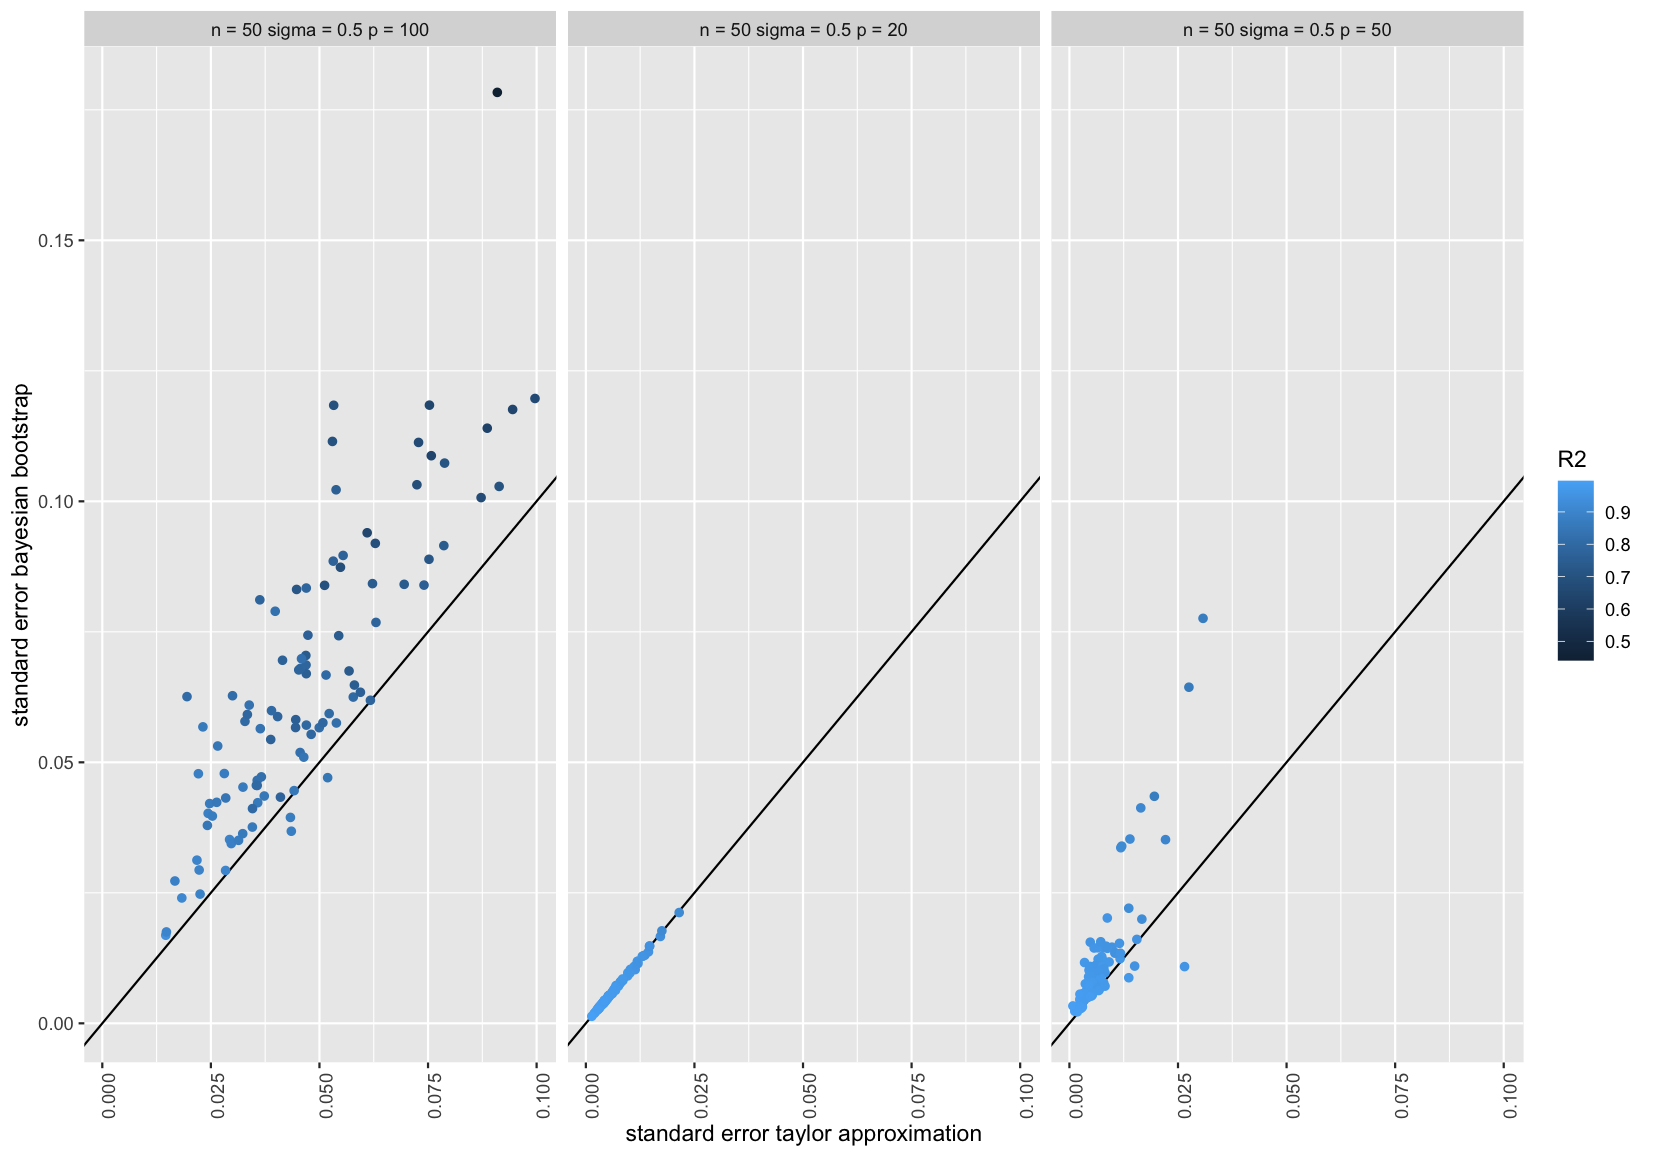
\includegraphics[width=\textwidth]{simres_high_p_n50.png}
    \caption{ Simulation results for high number of predictors.}
    \label{fig:simres_high_p}
\end{figure}

\newpage
\bibliographystyle{plainnat}
\bibliography{references.bib}

\end{document}